\documentclass[a4paper, twocolumn]{article}


% you can switch between these two (and more) styles by commenting one out (use percentage)
\usepackage[backend=biber]{biblatex}
%\usepackage[backend=biber, style=authoryear-icomp]{biblatex}
\addbibresource{./refs.bib}

\usepackage{graphicx}
\graphicspath{{./images/}}

\usepackage{listings}
\usepackage{color}

\usepackage{tabularx}
\definecolor{lightgray}{gray}{0.9}

% code listing: https://tex.stackexchange.com/questions/19004/how-to-format-an-inline-source-code
\lstset{
    showstringspaces=false,
    basicstyle=\ttfamily,
    keywordstyle={blue},
    commentstyle=\color[gray]{0.6}
    stringstyle=\color[RGB]{255, 150, 75}
}
\newcommand{\inlinecode}[2]{\colorbox{lightgray}{\lstinline[language=#1]$#2$}}

\author{Anton Kamenov, Cristian Guba, Stefanos Agelastos}
\title{Chicago Crime Rates Prediction}



\begin{document}

\twocolumn[
    \begin{@twocolumnfalse}
        \maketitle
        \begin{abstract}
            By using a data-driven approach this research focuses on exploring the crime rates
            in Chicago from year 2012 to 2016 in order to find a matching pattern for crime prediction in the future.
            The primary goal of this reasearch is to predict the amount of crime, based on the date and place.
            Using strong machine learning models it was possible to predict the crime rate. However, due to the low
            accuracy of the predictions it was concluded that it is not possible to rely solely on the models produced by this research
        \end{abstract}
    \end{@twocolumnfalse}
    \vspace{1cm}
]
\onecolumn

\tableofcontents

\newpage

\listoffigures

\newpage
\twocolumn

\section{Introduction\label{sec:Introduction}}

Crime has always been a major problem in small and big cities around the world.
Throughout the years, society has been trying to reduce the number of unlawful acts committed by people.
By establishing new rules and punishments for those who do not obey the law, people have found a way to reduce the crime rate.
Nations have evolved their legal systems during thousands of years of trial and error, but that still does not stop citizens from commiting a crime.

There are many reasons why people still tend to participate in unlawful activities. 
Whether it be because of poor living conditions, psychological disorders or other, the world is always going to be a witness of crimes, no matter how scary the consecuenses of committing them are.
For this reason the safety of each city is handed over to the police departments.

Police departments are another tool for lowering the amount of crimes.
They operate by answering to people's calls for help and by patrolling around the city, split into designated areas.
Sometimes, however, there are not enough patroling cars in the area to react quickly to the amount of crimes happening at the same time.

\section{Research Question}
By collecting data from one of the U.S's largest cities - Chicago,
where the murder rate has remained persistently high troughout the years\cite{friedman2017crime},
this reasearch is going to use a data-driven approach to examine if:
\begin{itemize}
    \item Crime is influenced by the date and time;
    \item Crime is influenced by the districts.
\end{itemize}
Using the analysis the reasearch is going to try to answer the question:
\begin{itemize}
    \item Can crime rate be predicted based on the date, time and disctrict?
\end{itemize}

\section{Methods}

This research objectives necessitate a multi-methodological approach that integrates theory building, systems development, observation and experimentation, as described by Nunamaker et al\cite{nunamaker1990systems}.
Rather than a linear research method, this approach can be considered an agile research model, due to the continuous going back and forth between theory building, systems development, observation, and experimentaion.

\subsection{Theory building}
\label{theorybuilding}
    Starting with the dataset\cite{dataset}, the research is going to begin with data exploration,
    in order to see how the data looks like. Viewing the different features the dataset has and the missing
    values, it will help to formulate a theory that will need to be proven.
    After removing or extrapolating the missing values, different parts of the data can be plotted in order
    to gain more insight into how the data is looking.
\subsection{System development}
\label{systemdevelopment}
    Next part is the System development, which involes creating new features to the dataset (feature engineering),
    converting one type of data to another (for example date and time to UNIX timestamp).
    After that models are selected for experimantation with the newly build data.
\subsection{Observation}
\label{observation}
    The Observation happens after each model is trained. By examining the result a decision needs to be made
    to choose  which model performs the best in the given conditions with the given parameters.
\subsection{Experimentation}
\label{experimentation}
    After observation the research is continued by making small adjustments to the model parameters and the dataset
    in order to see what changes will take place and how will they influence the results.

\section{Analysis}
\subsection{Data Cleanup and data exploration}
With the process described in section \ref{theorybuilding} the research started by analyzing the content of the dataset. 
Non-relevant rows were dropped in order to gain more focus on data related to place and time. 
There are some specific days during which the crime rate is significantly higher, which mostly corresponds to most popular national holidays. 
During daytime, the crime rate in Chicago is lower and the number of the most dangerous crime types tend to increase during the night. 
As can be seen in Figure 1, there is a specific pattern for each year - seasonality, for how the number of crimes changes every month. 
There is also a trend observed, where the number of crimes is decreasing every year. 
\begin{figure}
    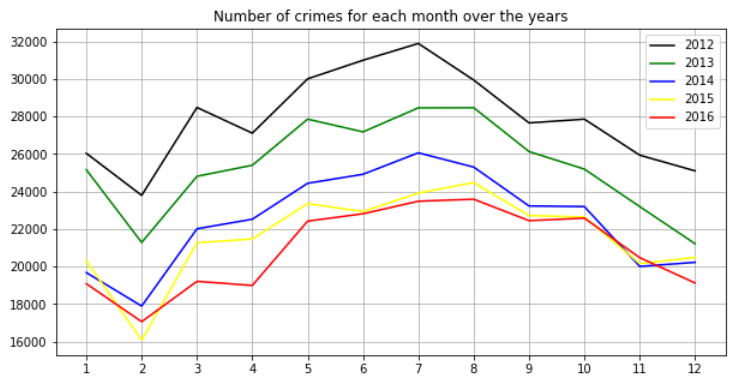
\includegraphics[scale=0.3]{fig1.png}

    \caption{Number of Crimes throughout the years}
\end{figure}

\begin{figure}
    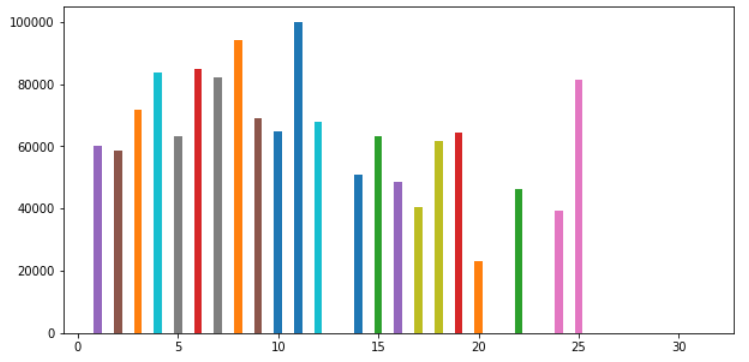
\includegraphics[scale=0.3]{fig2.png}
    \caption{Number of crimes for each district}
\end{figure}
The city is divided into 22 police districts, this parameter was chosen as a feature for the location of the crime.
After the graphical representation of the number of crimes in each district in Figure 2
it is possible to identify that there are districts with a higher number of crime count. 
This doesn’t mean that a specific district should have a higher level of alarm as each district is of different size and different number of population.

For the date and time columns some aditional cleanup steps were implemented. 
The date and time was converted to a UNIX timestamp. This was chosen so that there is continuity in the feature, turning date and time into a discrete numerical parameter.  
Each timestamp represents an hour of the day for the specific day.
By aggregating the number of crimes for each hour in a specific district, a new feature is created holding the count of crimes(Section \ref{systemdevelopment}).

\subsection{Time Series Analysis}
For the timeseries analysis and forecasting, the chosen ARIMA model is expecting a series of monodimentional, periodic data. 
In order to accomodate the model we removed the district feature and aggregated the crime count based on the timestamp.
One can see the daily crime count for the peak months of Spring and Summer 2015 
in Figure 8 of the Appendix \ref{appendix:fig3}. 
It is noticeable that there are outliers on the first day of every month. 
It is uncertain if that is a systematic error, or an actual occurence so this poses an interesting problem. 
By choosing a weekly forecasting period, the outlier values of the first day were spread over the first week of each month 
(Figure 9 of Appendix \ref{appendix:fig4}) smoothing out the outlier values.

\subsection{Splitting the set in training, validation and testing sets}\label{split}
In order to train the models, tune their hyperparameters and test the results on unseen data the dataset is cleaned and split in 3 sub sets.
The data is split in chronological order, where the training set is chronologically first, the validation set comes next and the test data is the last. 
The reason is that the research questions are trying to get answers about unknown future values – extrapolation. 
The aim is to train and evaluate the models in a chronological order, by learning on previous data and forecasting future uknown data. 
For the timeseries ARIMA model, the data is split in 75\% train/validation and 25\% test data, then the train/validation is further split in 75\% train and 25\% validation. 
For the rest of the machine learning models, the split is 60\% training, 20\% validation and 20\% testing.

\begin{flushleft}
    \begin{tabular}{ c c }
        Timeseries Dataset:\\
        Size of Training set &    : (147)\\
        Size of Validation set &  : (49)\\
        Size of Test set &        : (65)\\
        Machine Learning Dataset  :\\
        Size of Training set X &  : (24147, 2)\\
        Size of Training set Y&   : (24147,)\\
        Size of Validation set X &: (8049, 2)\\
        Size of Validation set Y& : (8049,)\\
        Size of Testing set X &   : (8049, 2)\\
        Size of Testing set Y&    : (8049,)\\

    \end{tabular}
\end{flushleft}

\subsection{Ridge Regressor model}
Using the already split training set and validation set, a Ridge Regressor model was trained in order to
try to predict the actual amount of crime for a specific time period and a specific district. Due to the shape of 
the data this experiment was not very successful.

\subsection{Implementation and Parameter tuning for ARIMA}\label{ARIMA}
Following the methods in Section \ref{systemdevelopment} the choice to include a classical forecasting model for timeseries seems natural, 
as these models are known in many cases to perform better, needing less data, as observed by Parmezanet al. \cite{test}
The Autoregresssive Integrated Moving Average (ARIMA) model is a good fit for this purpose due to the observed trend in the dataset, Figure 2.
The ARIMA model is a common choice for this type of datasets, as seen in similar works by Al Balamesh et al and Eymen et al. \cite{one} \cite{two} 
The model hyperparameters are initialising the three different aspects of ARIMA, \textbf{p} for autoregression, \textbf{d} integration and \textbf{q} for the moving average. 
The Grid Search method was used, as described by LaValle et al, \cite{lavalle2004relationship} and walk-forward train/validation steps were executed for each combination of the selected hyperparameter values(\ref{experimentaion}). 
The Mean Square Error was used in order to evaluate and compare the predictions for each hyperparameter set (Section \ref{observation}).

\subsection{Implementation and Parameter Tuning for Decision Tree Classifier}
Further in the analysis it was found that the existing data is very clustered, as can be seen in Figure 3

\begin{figure}[h]
    \label{figure:}
    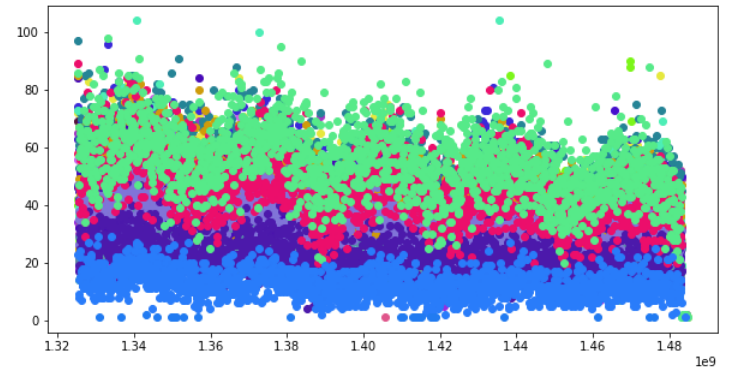
\includegraphics[scale=0.3]{fig5.png}
    \caption{All crimes for each Disctict during the years 2012-2016}
\end{figure}

This type of data would indicate that using a regression model to predict the amount of crimes would not be a good fit.
For this reason a classifier model would be a better fit for this dataset.
In order to create and use a Decision Tree Classifier a new feature needed to be created for the dataset which
would classify the amount of crimes for each day into 3 groups:
\begin{enumerate}
    \item \textbf{Low Crime Rate - 0}
    \item \textbf{Medium Crime Rate - 1}
    \item \textbf{High Crime Rate - 2}
\end{enumerate}
By observing the dataset it was found that the median value for the amount of crimes is 35 which will be the border between the
\textbf{Low Crime Rate} and \textbf{Medium Crime Rate}. The next partition will be at 50. Every crime rate that is above 35 and 
below 50 will be classified as \textbf{Medium Crime Rate}. Everything above 50 and below 104(the maximum amount of crimes recorded)
is classified as \textbf{High Crime Rate}.

Using the methods in Section \ref{split} the new train, validation and test sets were created in order to train a Decision Tree Classifier.
Grid search cross validation over specified parameter values  was implemented in order to tune the decision tree  model to the best performance.
The hyper-parameters used for the search were:
\begin{enumerate}
    \item \textbf{Maximum Depth - 2, 3, 5, 10, 20}
    \item \textbf{Minimun Samples per leaf - 5, 10, 20, 50, 100}
    \item \textbf{Criterion - gini, entropy}
\end{enumerate}

This way the model will be tested with each of the parameters provided and increase the accuracy of the predictions.

\section{Findings}
The regression model did not perform well in this research. The overall accuracy of the model was 18\% which is not
really useful in any scenario.

\begin{figure}[h]
    \label{figure:}
    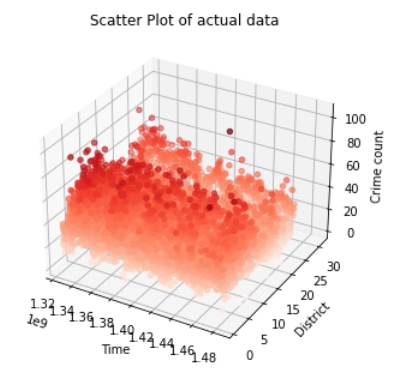
\includegraphics[scale=0.3]{fig7.png}
    \caption{The data used for testing}
\end{figure}

\begin{figure}[h]
    \label{figure:}
    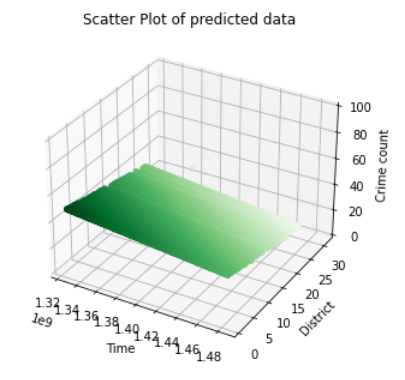
\includegraphics[scale=0.3]{fig8.png}
    \caption{Predicted data}
\end{figure}


\begin{figure}[h]
    \label{figure:}
    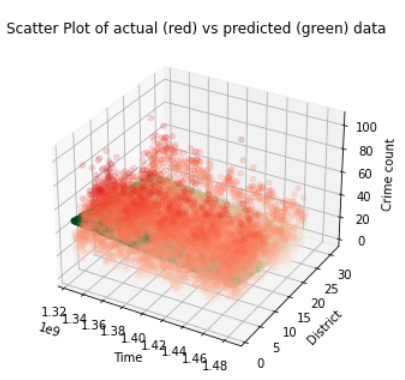
\includegraphics[scale=0.3]{fig9.png}
    \caption{Predicted data vs Actual data}
\end{figure}

The Figures above show the differences between the actual data and the predicted data. The model is linear, 
so the predicted values form a plane, while the shape of the observations have curves and don't really shape a surface. It can 
be clearly seen that the model is underfitting and not suited for this data set.
For these reasons we did not move forward with hyperparameter tuning for the Linear Ridge Regressor.

The results of the Grid Search method for selecting ARIMA hyperparemeter values resulted to an ARIMA(4, 0, 0) 
with a Mean Square Error of 136 179 for the train/validation sets and 84 182 for the test set. 
This means that according to this research a simple Auto Regressive model with a lag order of 4 is enough, as values of 0 
for the Integration and Moving Average are disabling these last two models. 
In Figure 7 of Appendix \ref{appendix:fig5} the results of the tuned model can be seen on the test data, and the actual observations.

The result from the decission tree classifier before the tuning had an accuracy of 64.02\%.
The following confusion matrix shows that the model guessed correctly mostly the crime rate classified as \textbf{Low}.

\begin{tabularx}{0.45\textwidth} { 
  | >{\raggedright\arraybackslash}X 
  | >{\centering\arraybackslash}X 
  | >{\centering\arraybackslash}X
  | >{\centering\arraybackslash}X | }
 \hline
 Predicted Rate & 0 & 1 & 2 \\
 \hline
 Actual Rate  &   &   &  \\
 \hline
 0  & 4610  &651   &45\\
 1  & 1695  &406  &191\\
 2  & 273   &41  &137\\
\hline
\end{tabularx}

Further analysis in the classification report shows that the precision is not so high for the Medium and High Alarm which are more important
in therms of accuracy.

\begin{tabularx}{0.48\textwidth} { 
    | >{\raggedright\arraybackslash}X 
    | >{\centering\arraybackslash}X 
    | >{\centering\arraybackslash}X
    | >{\centering\arraybackslash}X
    | >{\centering\arraybackslash}X | }
   \hline
    &precision&recall&f1-score&support\\
   \hline
    0&0.70&0.87&0.78&5306\\
    \hline
    1&0.37&0.18&0.24&2292\\
    \hline
    2&0.37&0.30&0.33&451\\
    \hline
    accuracy&&&0.64&8049\\
    \hline
    macro avg&0.48&0.45&0.45&8049\\
    \hline
    weighted avg&0.59&0.60&0.60&8049\\
    \hline
  \end{tabularx}

By tuning the Classifier using Grid Search it turned out that the following parameters are the best for this type of classification.
\begin{itemize}
    \item Maximun depth = 10;
    \item Minimun samples per leaf = 100;
    \item Random state = 42;
\end{itemize}

The accuracy went up to 0.71\%.

The classification report shows that although the accuracy went slightly up, the most important predictions(Medium and High Crime rate) are still
low on the scale.

\begin{tabularx}{0.5\textwidth} { 
    | >{\raggedright\arraybackslash}X 
    | >{\centering\arraybackslash}X 
    | >{\centering\arraybackslash}X
    | >{\centering\arraybackslash}X
    | >{\centering\arraybackslash}X | }
   \hline
    &precision&recall&f1-score&support\\
   \hline
    0&0.79&0.87&0.83&5306\\
    \hline
    1&0.53&0.42&0.47&2292\\
    \hline
    2&0.37&0.30&0.33&451\\
    \hline
    accuracy&&&0.71&8049\\
    \hline
    macro avg&0.56&0.53&0.54&8049\\
    \hline
    weighted avg&0.69&0.71&0.70&8049\\
    \hline
  \end{tabularx}

\section{Conclusion}
Based on this research, it can be concluded that time and place are factors which influence the number and type of crimes in a specific district, 
which could help police to distribute their resources better by planning where and how many officers should be deployed to patrol. 
Is this information enough for an artificial intelligence model to predict where and which type of crime could happen? 
Clearly not, as the behavior of human beings is not so easy to predict, usually it is influenced by a lot of external factors which are very important and not included in our data. 
Covid-19 was a factor that changed people's behavior and their mental health \cite{kim2021exploring}. Therefore, crime amount and their types changed significantly during lockdowns. 
Restrictions also caused limitations in people's movement. Using such models to predict crime poses some serious ethical questions,
as this is a very sensitive subject. Current generations tend to prioritize human life and the job of the state is to protect it.

\onecolumn
\printbibliography[heading=bibintoc,title={Bibliography}]
\newpage

\appendix

\section{Appendix}


\subsection{Figure 7 - ARIMA test set results}\label{appendix:fig5}
\begin{figure}[h]
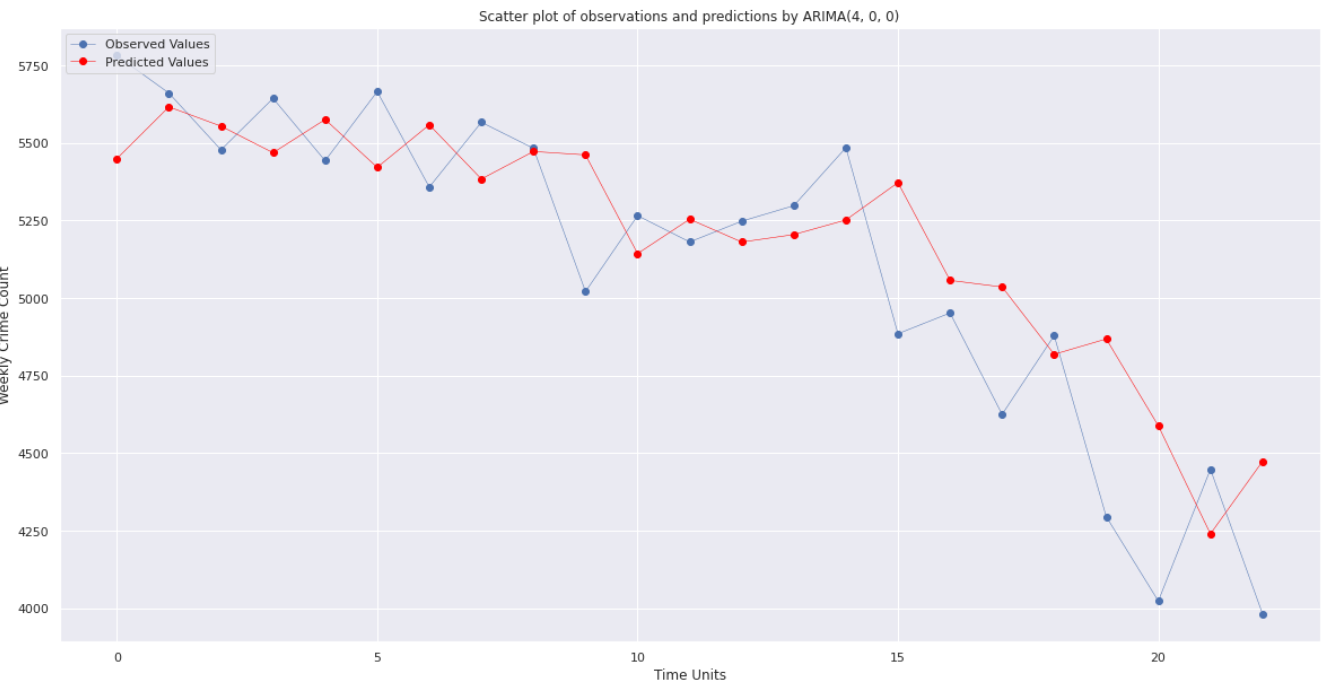
\includegraphics[width=\textwidth]{fig6.png}
\caption{Test set observations and ARIMA forecasting}
\end{figure}
\newpage

\subsection{Figure 8 - Spring and Summer 2015 daily Crime count}\label{appendix:fig3}
\begin{figure}[h]
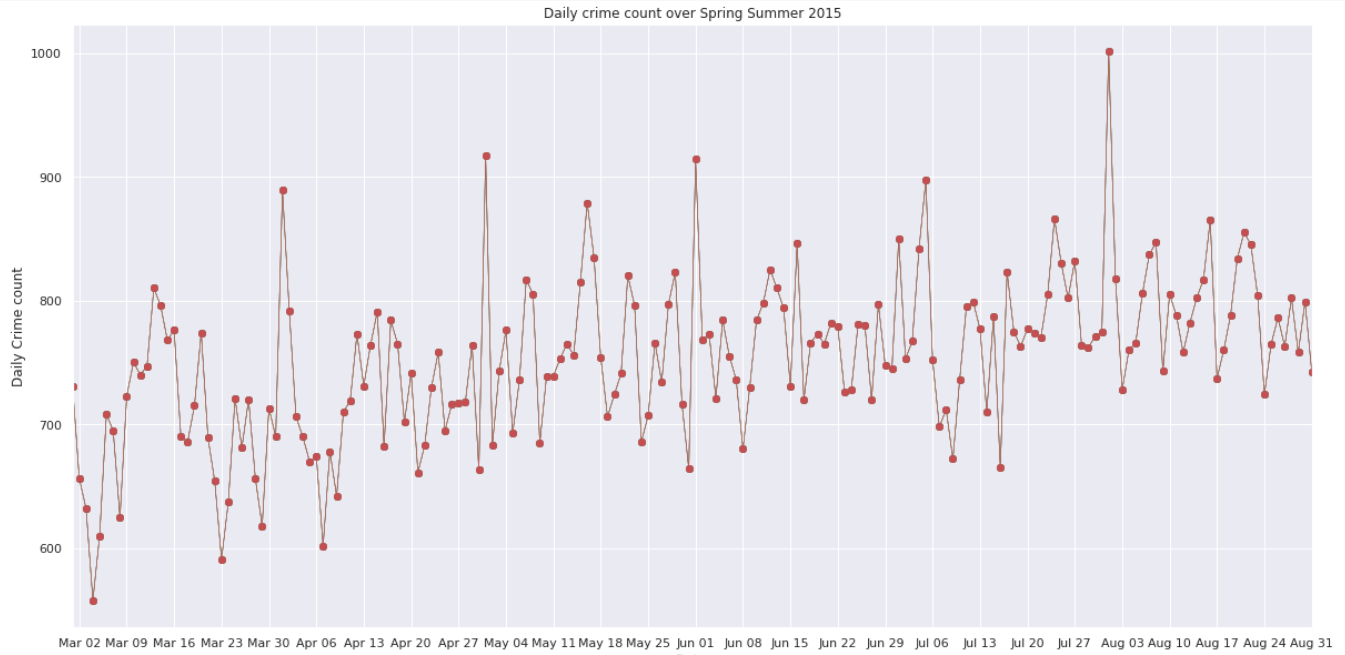
\includegraphics[width=\textwidth]{fig3.png}
\caption{Spring and Summer 2015 daily Crime count}
\end{figure}
\newpage

\subsection{Figure 9 - Spring and Summer 2015 weekly Crime count}\label{appendix:fig4}
\begin{figure}[h]
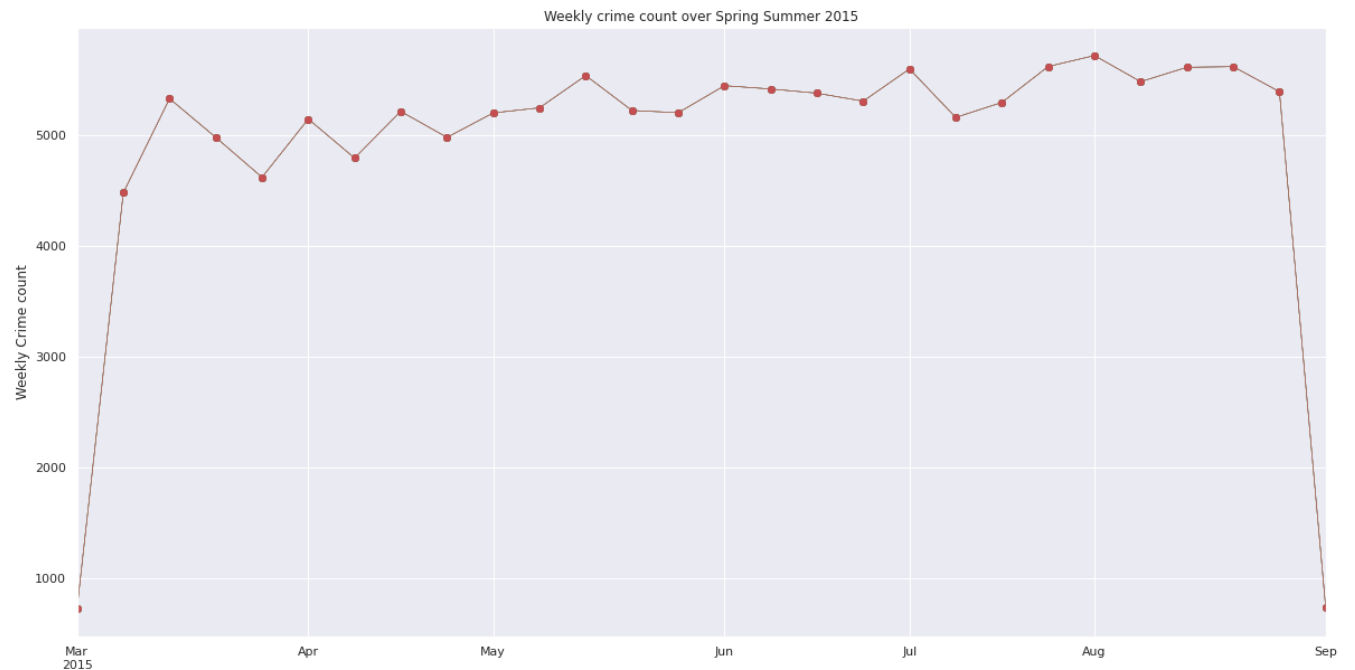
\includegraphics[width=\textwidth]{fig4.png}
\caption{pring and Summer 2015 weekly Crime count}
\end{figure}

\end{document}
